\begin{frame}{Newton iteration: workhorse of SNES}
  \begin{textblock}{3}(11,0)
    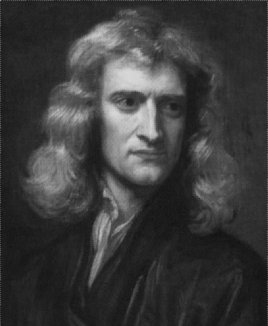
\includegraphics[width=\textwidth]{figures/Newton}
  \end{textblock}
  \begin{itemize}
  \item Standard form of a nonlinear system
    \[ F(u) = 0 \]
  \item Iteration
    \begin{align*}
      \text{Solve:} & \qquad J(u) w = -F(u) \\
      \text{Update:} & \qquad u^+ \gets u + w
    \end{align*}
    \item Quadratically convergent near a root: $\abs{u^{n+1}-u^*} \in \bigO\Big(\abs{u^n-u^*}^2\Big)$
    \item Picard is the same operation with a different $J(u)$
  \end{itemize}
  \begin{example}[Nonlinear Poisson]
    \begin{align*}
      F(u)=0 \quad &\sim\quad -\div\big[ (1+u^2) \nabla u \big] - f = 0 \\
      J(u)w \quad &\sim\quad  -\div\big[(1+u^2)\nabla w + 2uw\nabla u \Big]
    \end{align*}
  \end{example}
  % \begin{example}[$\pp$-Bratu]
  %   Suppose $F$ is a discretization of
  %   \[ -\nabla \cdot \big( \eta \nabla u \big) - \lambda e^u - f = 0 \]
  %   \[\eta(\gamma) = (\epsilon^2+\gamma)^{\frac{\pfrak-2}{2}}, \qquad\quad \gamma = \half \abs{\nabla u}^2. \]
  %   Then $J(u)w$ is a discretization of
  %   \[ -\nabla \cdot \big( \eta \nabla w + \eta' (\nabla u \cdot \nabla w)\nabla u \big) - \lambda e^{u} w . \]
  % \end{example}
\end{frame}

